\documentclass[15pt,a5paper,reqno]{article}
\usepackage{hyperref}
\usepackage[warn]{mathtext}
\usepackage[utf8]{inputenc}
\usepackage[T2A]{fontenc}
\usepackage[russian]{babel}
\usepackage{amssymb, amsmath, multicol}
\usepackage{graphicx}
\usepackage[shortcuts,cyremdash]{extdash}
\usepackage{wrapfig}
\usepackage{gensymb}
\usepackage{floatflt}
\usepackage{lipsum}
\usepackage{verbatim}
\usepackage{concmath}
\usepackage{euler}
\usepackage{xcolor}
\usepackage{etoolbox}
\usepackage{fancyhdr}
\usepackage{subfiles}
\usepackage{enumitem}
\usepackage{amsthm}
\usepackage{indentfirst}
\usepackage{import}
\usepackage{multirow}
\usepackage{hhline}
\usepackage{calrsfs}

\DeclareMathOperator{\sign}{sign}

\RequirePackage[ left     = 1cm,
                 right    = 1cm,
                 top      = 2.0cm,
                 bottom   = 1.25cm,
                 includefoot,
                 footskip = 1.25cm ]{geometry}
                 
\setlength{\parskip}{ .5em plus .15em minus .08em }
\renewcommand {\baselinestretch}{ 1.07 }

\fancyhf{} % clear existing header/footer entries

\renewcommand{\footrulewidth}{ .0em }
\fancyfoot[C]{\texttt{\textemdash~\thepage~\textemdash}}

\makeatletter
\patchcmd\l@section{%
  \nobreak\hfil\nobreak
}{%
  \nobreak
  \leaders\hbox{%
    $\m@th \mkern \@dotsep mu\hbox{.}\mkern \@dotsep mu$%
  }%
  \hfill
  \nobreak
}{}{\errmessage{\noexpand\l@section could not be patched}}
\makeatother
\parindent = 1cm % отступ при красной строке⏎
\pagestyle{fancy}    
\renewcommand\qedsymbol{$\blacksquare$}

\newcommand{\when}[2]{
  \left. #1 \right|_{#2} \hspace
}
\renewcommand{\kappa}{\varkappa}
\RequirePackage{caption2}
\renewcommand\captionlabeldelim{}
\newcommand*{\hm}[1]{#1\nobreak\discretionary{}

\DeclareSymbolFont{T2Aletters}{T2A}{cmr}{m}{it}
{\hbox{$\mathsurround=0pt #1$}}{}}
% Цвета для гиперссылок
\definecolor{linkcolor}{HTML}{000000} % цвет ссылок
\definecolor{urlcolor}{HTML}{799B03} % цвет гиперссылок
 
\hypersetup{pdfstartview=FitH,  linkcolor=linkcolor,urlcolor=urlcolor, colorlinks=true}


\begin{document}

% НАЧАЛО ТИТУЛЬНОГО ЛИСТА
\begin{center}
  {\small ФЕДЕРАЛЬНОЕ ГОСУДАРСТВЕННОЕ АВТОНОМНОЕ ОБРАЗОВАТЕЛЬНОЕ\\ УЧРЕЖДЕНИЕ ВЫСШЕГО ОБРАЗОВАНИЯ\\ МОСКОВСКИЙ ФИЗИКО-ТЕХНИЧЕСКИЙ ИНСТИТУТ\\ (НАЦИОНАЛЬНЫЙ ИССЛЕДОВАТЕЛЬСКИЙ УНИВЕРСИТЕТ)\\ ФИЗТЕХ-ШКОЛА РАДИОТЕХНИКИ И КОМПЬЮТЕРНЫХ ТЕХНОЛОГИЙ}\\
  \hfill \break
  \hfill \break
  \hfill \break
  \Huge{Работа 3.7.1. \\ Скин-эффект в полом цилиндре}\\
\end{center}

\hfill \break
\hfill \break
\hfill \break
\hfill \break
\hfill \break
\hfill \break
\hfill \break
\hfill \break

\begin{flushright}
  \normalsize{Работу выполнил:}\\
  \normalsize{\textbf{Долгов Александр Алексеевич, группа Б01-106}}\\
\end{flushright}

\begin{center}
  \normalsize{\textbf{Долгопрудный, 2022}}
\end{center}

\thispagestyle{empty} % выключаем отображение номера для этой страницы

% КОНЕЦ ТИТУЛЬНОГО ЛИСТА

\newpage
\thispagestyle{plain}
\tableofcontents
\thispagestyle{plain}
\newpage

\section{Аннотация}

    В данной работе изучается скин-эффект в длинном тонкостенном медном цилиндре, помещённом внутрь соленоида.
	
\section{Теоретические сведения}

    \begin{wrapfigure}{r}{0.3\textwidth}
        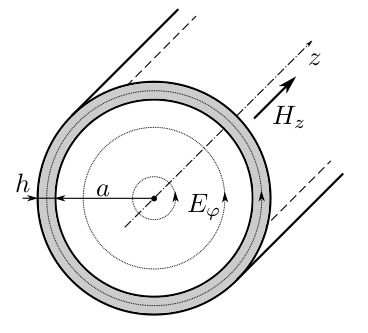
\includegraphics[width=0.3\textwidth]{images/picture_1.png}
        \textbf{Рис. 1. Поля в тонкостенном цилиндре}
    \end{wrapfigure}
    Пусть цилиндр настолько длинный, что в нём можно пренебречь краевыми эффектами. В таком случае внутри цилиндра $\vec H$ направлен вдоль оси системы, а вихревое электрическое поле $\vec E$ всюду перпендикулярно ей. Будем считать, что все величины изменяются по гармоническому закону с частотой $\omega$, равной частоте колебаний тока в соленоиде. Тогда:
    \begin{equation}\label{fields}
    \begin{split}
        H_z = H(r)e^{i\omega t}\\
        E_{\varphi} = E(r)e^{i\omega t}
    \end{split}
    \end{equation}
    Так как на границе цилиндра должны быть непрерывны касательные компоненты $\vec E$ и $\vec B$, то функции $E(r)$ и $H(r)$ непрерывны по всей исследуемой области.

    Пусть длинный полый цилиндр имеет радиус $a$ и толщину стенки $h \ll a$ (последнее условие позволяет описывать поле внутри стенки как одномерное). Так как в полости цилиндра ток отсутствует, то магнитное поле в ней однородно (как и поле внутри пустого соленоида). Из этого следует:
    \begin{equation*}
        H_z(r, t) = H_1e^{i\omega t},\\\ 0 \leq r \leq a
    \end{equation*}
    где $H_1$ - амплитуда напряжённости магнитного поля на внутренней поверхности цилиндра. По закону электромагнитной индукции:
    \begin{equation*}
        E_{\varphi}\cdot 2\pi r = -\pi r^2 \frac{dB_z}{dt} = -\mu_0 \pi r^2 \frac{dH_z}{dt} \implies E(r) = -\frac{\mu_0}{2}\cdot i\omega H_1
    \end{equation*}
    Отсюда получаем связь для амплитуд полей на внутренней поверхности цилиндра:
    \begin{equation*}
        E_1 = -\frac{i}{2}\mu_0\omega aH_1
    \end{equation*}

    \hypertarget{pic_2}{\begin{wrapfigure}{l}{0.3\textwidth}
        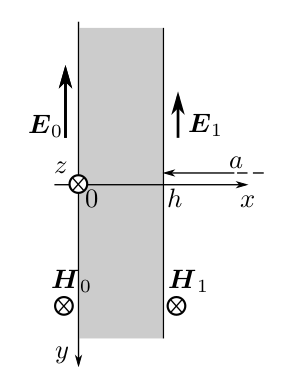
\includegraphics[width=0.3\textwidth]{images/picture_2.png}
        \textbf{Рис. 2. Поля в стенке цилиндра}
    \end{wrapfigure}}
    Поле внутри стенки цилиндра описывается уравнением скин-эффекта:
    \begin{equation*}
    \begin{split}
        \nabla^2 \vec H = \sigma\mu\mu_0 \frac{\partial \vec H}{\partial t} \\
        \nabla^2 \vec E = \sigma\mu\mu_0 \frac{\partial \vec E}{\partial t}
    \end{split}
    \end{equation*}
    которое в одномерном случае имеет вид (нас будет интересовать уравнение только для магнитного поля):
    \begin{equation}\label{se_equation}
        \frac{\partial^2 H_z}{\partial x^2} = \sigma \mu\mu_0\frac{\partial H_z}{\partial t},
    \end{equation}
    где $\sigma$ - удельная проводимость, направление оси указано на \hyperlink{pic_2}{Рис. 2}. Пусть внутри стенок цилиндра поля описываются функциями \eqref{fields} c заменой $r$ на $x$. Тогда подстановка \eqref{fields} в \eqref{se_equation} даёт:
    \begin{equation*}
        \frac{d^2H(x)}{dx^2} = i\mu\mu_0\omega\sigma H(x)
    \end{equation*}
    Так как в работе используется медный цилиндр, то с высокой точностью можно считать, что $\mu = 1$. Тогда:
    \begin{equation}\label{diff_eq}
        \frac{d^2H(x)}{dx^2} = i\mu_0\omega\sigma H(x)
    \end{equation}
    Граничные условия для \eqref{diff_eq} зададим так:
    \begin{equation}\label{condition_1}
        H(x = 0) = H_0
    \end{equation}
    \begin{equation}\label{condition_2}
        H(x = h) = H_1
    \end{equation}
    где $H_0$ - амплитуда колебаний магнитного поля на внешней поверхности цилиндра. Решение \eqref{diff_eq} ищем в виде:
    \begin{equation}\label{solution}
        H(x) = Ae^{\alpha x} + Ce^{-\alpha x}
    \end{equation}
    Подставив \eqref{solution} в \eqref{diff_eq}, получим:
    \begin{equation*}
        \alpha^2 = i\mu\mu_0\omega\sigma \implies \alpha = \pm (i + 1)\sqrt{\frac{\mu\mu_0\omega\sigma}{2}}
    \end{equation*}
    Введём величину:
    \begin{equation*}
        \boxed{\delta = \sqrt{\frac{2}{\mu\mu_0\omega\sigma}}} - \text{глубина проникновения},\\\ [\delta] = \text{м}
    \end{equation*}
    Тогда:
    \begin{equation*}
        \alpha = \pm \frac{(i + 1)}{\delta}
    \end{equation*}
    Применим граничное условие \eqref{condition_1}:
    \begin{equation*}
        H_0 = A + C \implies A = H_0 - C
    \end{equation*}
    \begin{equation}\label{nearly_H}
        H(x) = H_0e^{\alpha x} - 2C\sh{\alpha x}
    \end{equation}
    По теореме о циркуляции магнитного поля:
    \begin{equation*}
        rot\vec H = \vec j = \sigma\vec E,
    \end{equation*}
    которая в одномерном случае имеет вид:
    \begin{equation*}
        \frac{\partial H_x}{\partial z} - \frac{\partial H_z}{\partial x} = \sigma E_y
    \end{equation*}
    В нашей задаче $H_x = 0$, поэтому:
    \begin{equation*}
        E_y = -\frac{1}{\sigma}\frac{dH_z}{dx} \implies -E(x)e^{i\omega t} = -\frac{1}{\sigma}\frac{dH}{dx}e^{i\omega t} \implies E(x) = \frac{1}{\sigma}\frac{dH}{dx}
    \end{equation*}
    \begin{equation*}
        E(x) = \frac{\alpha}{\sigma}(H_0 e^{\alpha x} - 2C\ch{\alpha x})
    \end{equation*}
    Теперь применим граничное условие \eqref{condition_2}:
    \begin{equation*}
        -\frac{i}{2}\mu_0\omega aH_1 = \frac{\alpha}{\sigma}(H_0 e^{\alpha h} - 2C\ch{\alpha h}) \implies 2C = \frac{1}{\ch{\alpha h}}\left(H_0 e^{\alpha h} + \frac{aH_1}{\alpha\delta^2}i\right)
    \end{equation*}
    Вспомним, что
    \begin{equation*}
        \alpha^2 = i\mu_0\omega\sigma = \frac{2i}{\delta^2} \implies \frac{i}{\delta^2} = \frac{\alpha^2}{2}
    \end{equation*}
    Отсюда:
    \begin{equation*}
        2C = \frac{1}{\ch{\alpha h}}\left(H_0 e^{\alpha h} + \frac{a\alpha}{2}H_1\right)
    \end{equation*}
    Подставим $2C$ в \eqref{nearly_H}:
    \begin{equation*}
        H_1 = H_0e^{\alpha h} - \frac{\sh{\alpha h}}{\ch{\alpha h}}H_0 e^{\alpha h} - \frac{\sh{\alpha h}}{\ch{\alpha h}}\frac{a\alpha}{2}H_1
    \end{equation*}
    \begin{equation*}
        H_1 = \frac{H_0}{\ch{\alpha h}} - \frac{\sh{\alpha h}}{\ch{\alpha h}}\frac{a\alpha}{2}H_1
    \end{equation*}
    \begin{equation*}
        \boxed{H_0 = H_1\left(\ch{\alpha h} + \frac{a\alpha}{2}\sh{\alpha h}\right)}
    \end{equation*}
    Рассмотрим предельные случаи:
    \begin{enumerate}
        \item $\delta \gg h$ (малые частоты)
            \begin{equation*}
                \alpha h = \pm(i + 1)\frac{h}{\delta} \implies |\alpha h| = \frac{h\sqrt{2}}{\delta} \ll 1 \implies \ch{\alpha h} \approx 1,\\\ \sh{\alpha h} \approx \alpha h
            \end{equation*}
            \begin{equation*}
                H_0 \approx H_1\left(1 + i\frac{ah}{\delta^2}\right)
            \end{equation*}
            \begin{equation}
                \frac{|H_0|}{|H_1|} = \sqrt{1 + \left(\frac{ah}{\delta^2}\right)^2} = \sqrt{1 + \frac{(\mu_0\omega\sigma ah)^2}{4}}
            \end{equation}
            При этом колебания $H_1$ отстают от колебаний $H_0$ на угол $\psi$, определяемые соотношением $\tg{\psi} = \frac{ah}{\delta^2}$.
            Заметим также, что:
            \begin{equation}\label{limit}
                \lim\limits_{\omega \rightarrow 0} \frac{|H_0|}{|H_1|} = 1
            \end{equation}
        \item $\delta \ll h$ (большие частоты)
            \begin{equation*}
                |\alpha h| = \frac{h\sqrt{2}}{\delta} \gg 1 \implies |\alpha a| \gg 1,\\\ \sh{\alpha h} \approx \ch{\alpha h} \approx \frac{e^{\alpha h}}{2}
            \end{equation*}
            \begin{equation*}
                H_0 = H_1\frac{a\alpha e^{\alpha h}}{4} = H_1\frac{a}{4\delta}(i + 1)e^{\frac{h}{\delta}(1 + i)} = H_1\frac{\sqrt{2}a}{4\delta}e^{i\frac{\pi}{4}}e^{\frac{h}{\delta}(1 + i)} = 
            \end{equation*}
            \begin{equation*}
                = H_1\frac{\sqrt{2}a}{4\delta}e^{\frac{h}{\delta}}e^{i\left(\frac{\pi}{4} + \frac{h}{\delta}\right)} = H_1\frac{\sqrt{2}a}{4\delta}e^{\frac{h}{\delta}}e^{i\left(\frac{\pi}{4} + \frac{h}{\delta}\right)}
            \end{equation*}
            Колебания $H_1$ отстают от колебаний $H_0$ на угол
            \begin{equation}\label{phase_shift}
                \psi = \frac{\pi}{4} + \frac{h}{\delta} = \frac{\pi}{4} + h\sqrt{\frac{\mu_0\omega\sigma}{2}}
            \end{equation}
    \end{enumerate}
        
\section{Экспериментальная установка}

    \hypertarget{pic_3}{\begin{wrapfigure}{l}{0.5\textwidth}
        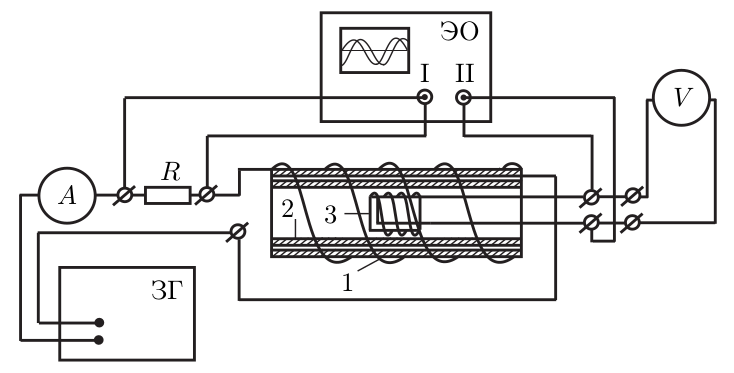
\includegraphics[width=0.5\textwidth]{images/picture_3.png}
        \textbf{Рис. 3. Экспериментальная установка}
    \end{wrapfigure}}

    Экспериментальная установка изображена на \hyperlink{pic_3}{рис. 3}. Переменное магнитное поле создаётся с помощью соленоида, намотанного на полый цилиндрический каркас 1 из поливинилхлорида, который подключается к генератору звуковой частоты ЗГ. Внутри соленоида расположен медный цилиндрический экран 2. Для измерения магнитного поля внутри экрана используется измерительная катушка 3. Действующее значение переменного тока в цепи соленоида измеряется амперметром $A$, а действующее значение напряжения на измерительной катушке измеряет вольтметр $V$. Для измерения
    сдвига фаз между током в цепи соленоида и напряжением на измерительной катушке используется двухканальный осциллограф. На вход одного канала подаётся напряжение с резистора $R$, которое пропорционально току, а на вход второго канала — напряжение с измерительной катушки.

\section{Методика измерений}

    \subsection{Измерение отношения амплитуд магнитного поля внутри и вне экрана}

        Вольтметром $V$ измеряется действующее значение ЭДС индукции, которая возникает в измерительной катушке 3, находящейся в магнитном поле с напряжённостью: $H(t) = H_1e^{i\omega t}$. Комплексную амплитуду ЭДС индукции найдём из закона электромагнитной индукции:
        \begin{equation*}
            \mathcal{E}_m = -SN\frac{dB_1(t)}{dt} = -i\omega\mu_0SNH_1e^{i\omega t},
        \end{equation*}
        где $S$ - площадь измерительной катушки, $N$ - число витков в ней. Тогда показания вольтметра, должны согласовываться с формулой:
        \begin{equation*}
            U = \mu_0\frac{SN\omega}{\sqrt{2}}|H_1| \implies |H_1| \propto \frac{U}{\nu}
        \end{equation*}
        При этом поле $H_0$ вне измерительной катушки пропорционально току $I$ в цепи соленоида, измеряемому амперметром $A$:
        \begin{equation*}
            |H_0| \propto I
        \end{equation*}
        Следовательно:
        \begin{equation}\label{fraction}
            \frac{|H_1|}{|H_0|} = \widetilde C \cdot \frac{U}{\nu I}
        \end{equation}
        Неизвестную константу, входящую в \eqref{fraction}, в силу \eqref{limit} можно найти измерениями при малых частотах как:
        \begin{equation*}
            \widetilde C = \lim\limits_{\nu \rightarrow 0} \frac{\nu I}{U}
        \end{equation*}

    \subsection{Определение проводимости материала экрана}
        В установке в качестве экрана используется медная труба промышленного производства. Технология изготовления труб оказывает заметное влияние на электропроводимость. Из-за наличия примесей проводимость меди трубы в установке отличается от табличного значения (в меньшую сторону). Для определения $\sigma$ экрана используется частотная зависимость \eqref{phase_shift} фазового сдвига между магнитными полями внутри и вне экрана при высоких частотах. 

        Из \eqref{phase_shift} видно, что при $\omega \gg (\mu_0 \sigma h^2)^{-1}$ зависимость $\psi(\sqrt{\omega})$ аппроксимируется прямой, проходящей через точку $\psi(0) = \frac{\pi}{4}$.
    
\section{Приборы и инструментальные погрешности}

    \noindent\textbf{Амперметр:}\\
        Абсолютная погрешность: $\sigma_I = 0.005\text{ мА}$

    \noindent\textbf{Вольтметр:}\\
        Абсолютная погрешность: $\sigma_U = 0.005\text{ мВ}$

    \noindent Погрешность измерения частоты тока в цепи соленоида считает пренебрежимо малой.

    \noindent Толщина экрана: $h = 1.5\text{ мм}$.
    
\section{Измерения и обработка их результатов}

    \subsection{Коэффициент ослабления магнитного поля}
        \noindentПолагая $\sigma \sim 5\cdot 10^7\ \frac{\text{См}}{\text{м}}$, находим, что частота, при которой $\delta = h$, равна
        \begin{equation*}
            \nu_h = \frac{1}{\pi\mu_0\sigma h^2} \approx 2250\text{ Гц}
        \end{equation*}
        Для удобства введём обозначение:
        \begin{equation*}
            \xi := \frac{U}{\nu I},\\\ [\xi] = \text{Ом}\cdot\text{с}
        \end{equation*}
        В области низких частот (от $\sim 0,01\nu_h$ до $\sim 0,1\nu_h$) было проведено 10 измерений действующих значений тока в цепи соленоида и ЭДС индукции в измерительной катушке. Результаты представлены в \hyperlink{table_1}{Таблице 1}. В этой же таблице приведены результаты вычислений величин $\frac{1}{\xi^2}$ и $\nu^2$. По этим значениям построен \hyperlink{graph_1}{График 1} зависимости $\frac{1}{\xi^2}(\nu^2)$. Экспериментальные точки аппроксимировались прямой $\frac{1}{\xi^2} = k_{\nu}^{(1)}\nu^2 + b_{\nu}^{(1)}$. В результате получено:
        \begin{equation*}
            b_{\nu}^{(1)} = (5.222 \pm 0.001)\cdot10^{-3}\frac{1}{\text{мОм}^2\cdot\text{с}^2}
        \end{equation*}
        Откуда находим:
        \begin{equation*}
            \xi_0^{(1)} = \frac{1}{\sqrt{b_{\nu}^{(1)}}} = (13.838 \pm 0.001)\ \text{мОм}\cdot\text{с}
        \end{equation*}

    \subsection{Проводимость материала экрана}

    Измерение проводимости материала экрана проводилось на основании формулы \eqref{phase_shift}. В связи с этим были проведены измерения сдвига фаз между магнитными полями $H_0$ и $H_1$ в области высоких частот (от $0.1\nu_h$ до $0.5\nu_h$). Результаты измерений приведены в \hyperlink{table_2}{Таблице 2}, по данным которой построен \hyperlink{graph_2}{График 2} зависимости $\psi(\sqrt{\omega})$. Экспериментальные точки аппроксимировались прямой $\psi = k\sqrt{\omega} + b$. В результате получено:
    \begin{equation*}
        |k| = (0.0115 \pm 0.0011)\sqrt{\text{с}}
    \end{equation*}
    По формуле \eqref{phase_shift} получаем:
    \begin{equation*}
        \sigma = \frac{2k^2}{\mu_0h^2} = 93.6\cdot10^6\ \frac{\text{См}}{\text{м}}
    \end{equation*}

    \subsection{Коэффициент ослабления поля}
    
    Найдём величину $\xi_0$ для области высоких частот. По данным таблицы 2 построен \hyperlink{graph_3}{График 3}. зависимости $\frac{1}{\xi^2}(\nu^2)$. Экспериментальные точки аппроксимировались прямой $\frac{1}{\xi^2} =k_{\nu}^{(2)}\nu^2 + b_{\nu}^{(2)}$. В результате получено:
     \begin{equation*}
        b_{\nu}^{(2)} = (4.96 \pm 0.05)\cdot10^{-3}\frac{1}{\text{мОм}^2\cdot\text{с}^2}
    \end{equation*}
    Откуда находим:
    \begin{equation*}
        \xi_0^{(2)} = \frac{1}{\sqrt{b_{\nu}^{(2)}}} = (14.20 \pm 0.07)\ \text{мОм}\cdot\text{с}
    \end{equation*}
    Для удобства введём обозначение:
    \begin{equation*}
        \beta := \frac{|H_1|}{|H_0|}
    \end{equation*}
    C учётом этого обозначения формула \eqref{fraction} приводится к виду:
    \begin{equation*}\label{weak_coeff}
        \beta = \frac{\xi}{\xi_0}
    \end{equation*}
    Значения $\beta$ для обеих серий измерений приведены в \hyperlink{table_4}{Таблице 4}. По этим данным построен \hyperlink{graph_4}{График 4}.
    
\section{Вывод}

    В процессе данной работы был изучен скин-эффект в длинном тонкостенном медном цилиндре, помещённом внутрь соленоида. Результаты эксперимента подтвердили, что магнитное поле ослабевает внутри проводника тем сильнее, чем выше частота изменения этого поля. Также найдена проводимость материала цилиндра. Полученное значение по порядку величины совпадает с табличным $(59.5\cdot10^6\ \frac{\text{См}}{\text{м}})$.
    
\newpage
\section{Приложения}

    \subsection{Таблицы}

    \noindent\hypertarget{table_1}{\textbf{Таблица 1. Область низких частот.}}
    \begin{center}
        \begin{tabular}{|c|c|c|c|c|}
        \hline
        U, мВ & I, мA & $\nu$, Гц & $\xi$, мОм $\cdot$ с & $\sigma_{\xi}$, мОм $\cdot$ с \\ \hline\hline
        134.5 & 435.4 & 22.5      & 13.729               & 0.005                      \\ \hline
        188.0 & 431.9 & 32.0      & 13.603               & 0.004                      \\ \hline
        241.2 & 427.5 & 42.0      & 13.434               & 0.003                      \\ \hline
        290.5 & 422.3 & 52.0      & 13.229               & 0.003                      \\ \hline
        335.6 & 416.5 & 62.0      & 12.996               & 0.002                      \\ \hline
        376.3 & 410.3 & 72.0      & 12.738               & 0.002                      \\ \hline
        412.7 & 404.0 & 82.0      & 12.458               & 0.002                      \\ \hline
        445.1 & 397.7 & 92.0      & 12.165               & 0.002                      \\ \hline
        473.8 & 391.6 & 102.0     & 11.862               & 0.002                      \\ \hline
        499.3 & 386.0 & 112.0     & 11.549               & 0.002                      \\ \hline
        \end{tabular}
    \end{center}

    \begin{center}
        \begin{tabular}{|c|c|c|}
        \hline
        $1/\xi^2$, $10^{-3}\cdot\text{мОм}^{-2}\cdot\text{с}^{-2}$ & $\sigma_{1/\xi^2}$, $10^{-3}\cdot\text{мОм}^{-2}\cdot\text{с}^{-2}$ & $\nu^2$, $\text{Гц}^2$ \\ \hline\hline
        5.305 & 0.004 & 506.25 \\ \hline
        5.404 & 0.003 & 1024   \\ \hline
        5.541 & 0.003 & 1764   \\ \hline
        5.714 & 0.002 & 2704   \\ \hline
        5.921 & 0.002 & 3844   \\ \hline
        6.163 & 0.002 & 5184   \\ \hline
        6.443 & 0.002 & 6724   \\ \hline
        6.757 & 0.002 & 8464   \\ \hline
        7.107 & 0.002 & 10404  \\ \hline
        7.497 & 0.002 & 12544  \\ \hline
        \end{tabular}
    \end{center}

    \newpage
    \noindent\hypertarget{table_2}{\textbf{Таблица 2. Область высоких частот.}}
    \begin{center}
        \begin{tabular}{|c|c|c|c|c|c|}
        \hline
        U, мВ & I, мA & $\nu$, Гц & $\xi$, мОм $\cdot$ с & $\sigma_{\xi}$, мОм $\cdot$ с & $\psi$, рад\\ \hline\hline
        674.5 & 322.9 & 324       & 6.447                & 0.001    & -1.082 \\ \hline
        682.8 & 311.9 & 424       & 5.1631               & 0.0009   & -1.198 \\ \hline
        681.0 & 303.7 & 524       & 4.2793               & 0.0008   & -1.307 \\ \hline
        674.0 & 296.5 & 624       & 3.6429               & 0.0007   & -1.375 \\ \hline
        664.1 & 289.7 & 724       & 3.1663               & 0.0006   & -1.434 \\ \hline
        651.7 & 282.9 & 824       & 2.7957               & 0.0005   & -1.467 \\ \hline
        637.7 & 275.9 & 924       & 2.5015               & 0.0005   & -1.513 \\ \hline
        621.7 & 268.4 & 1024      & 2.2620               & 0.0005   & -1.545 \\ \hline
        593.9 & 256.1 & 1200      & 1.9325               & 0.0004   & -1.547 \\ \hline
        \end{tabular}
    \end{center}

    \begin{center}
        \begin{tabular}{|c|c|c|}
        \hline
        $1/\xi^2$, $10^{-3}\cdot\text{мОм}^{-2}\cdot\text{с}^{-2}$ & $\sigma_{1/\xi^2}$, $10^{-3}\cdot\text{мОм}^{-2}\cdot\text{с}^{-2}$ & $\nu^2$, $\text{Гц}^2$ \\ \hline\hline
        24.056 & 0.05 & 104976 \\ \hline
        37.51  & 0.07 & 179776   \\ \hline
        54.61  & 0.08 & 274576   \\ \hline
        75.4   & 0.1  & 389376   \\ \hline
        99.7   & 0.1  & 524176   \\ \hline
        127.9  & 0.1 & 678976   \\ \hline
        159.8  & 0.2 & 853776   \\ \hline
        195.4  & 0.2 & 1048576   \\ \hline
        \end{tabular}
    \end{center}

    \newpage
    \noindent\hypertarget{table_3}{\textbf{Таблица 3. Коэффициент ослабления магнитного поля.}}
    \begin{center}
        \begin{tabular}{|c|c|c|c|}
            \hline
            $\xi$, мОм $\cdot$ с & $\sigma_{\xi}$, мОм $\cdot$ с & $\beta$ & $\sigma_{\beta}$ \\ \hline
            \hline
            13.729               & 0.005  & 0.9922 & 0.0004 \\ \hline
            13.603               & 0.004  & 0.9830 & 0.0003 \\ \hline
            13.434               & 0.003  & 0.9708 & 0.0002 \\ \hline
            13.229               & 0.003  & 0.9560 & 0.0002 \\ \hline
            12.996               & 0.002  & 0.9392 & 0.0002 \\ \hline
            12.738               & 0.002  & 0.9205 & 0.0002 \\ \hline
            12.458               & 0.002  & 0.9003 & 0.0002 \\ \hline
            12.165               & 0.002  & 0.8791 & 0.0002 \\ \hline
            11.862               & 0.002  & 0.8572 & 0.0002 \\ \hline
            11.549               & 0.002  & 0.8346 & 0.0001 \\ \hline
            \hline
            6.447                & 0.001    & 0.454  & 0.002  \\ \hline
            5.1631               & 0.0009   & 0.364	 & 0.002  \\ \hline
            4.2793               & 0.0008   & 0.301  & 0.001  \\ \hline
            3.6429               & 0.0007   & 0.257  & 0.001  \\ \hline
            3.1663               & 0.0006   & 0.223  & 0.001  \\ \hline
            2.7957               & 0.0005   & 0.197  & 0.001  \\ \hline
            2.5015               & 0.0005   & 0.1762 & 0.0009 \\ \hline
            2.2620               & 0.0005   & 0.1593 & 0.0008 \\ \hline
            1.9325               & 0.0004   & 0.1361 & 0.0007 \\ \hline
        \end{tabular}
    \end{center}

    \newpage
    \subsection{Графики}

    \noindent\hypertarget{graph_1}{\textbf{График 1.}}
    \begin{center}
        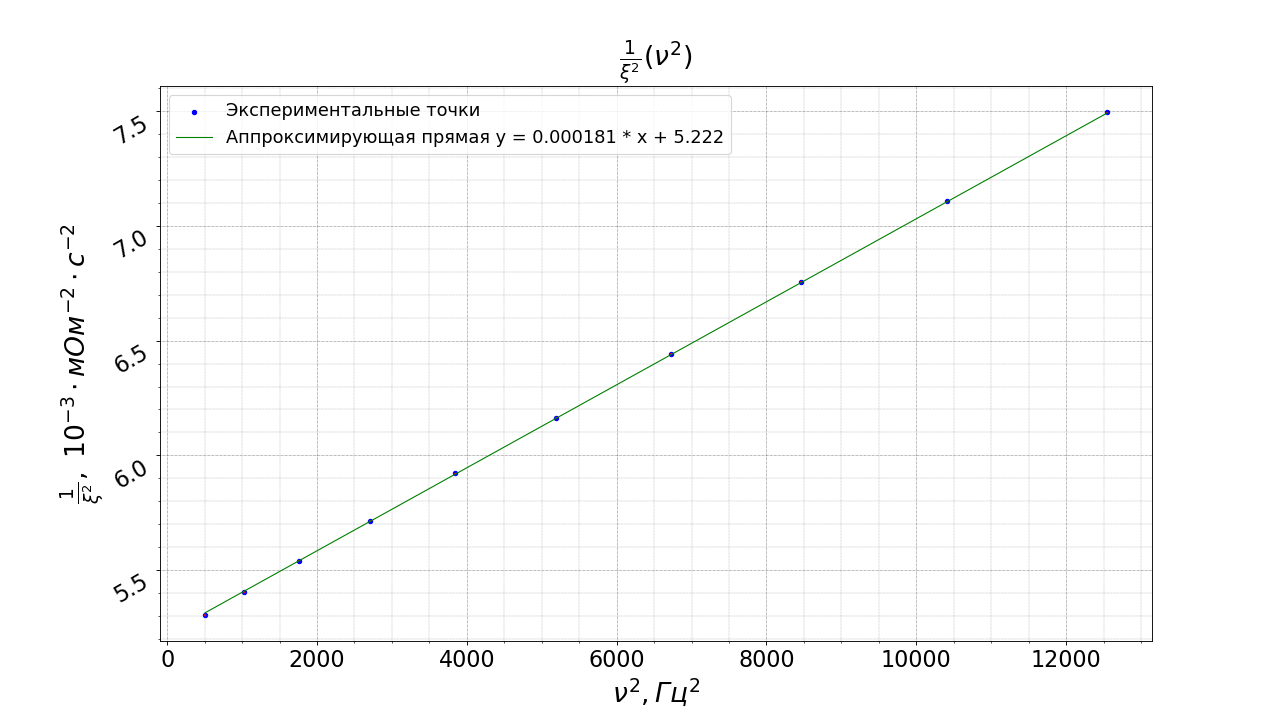
\includegraphics[width = 0.9\textwidth]{images/graph_1.png}
    \end{center}

    \noindent\hypertarget{graph_2}{\textbf{График 2.}}
    \begin{center}
        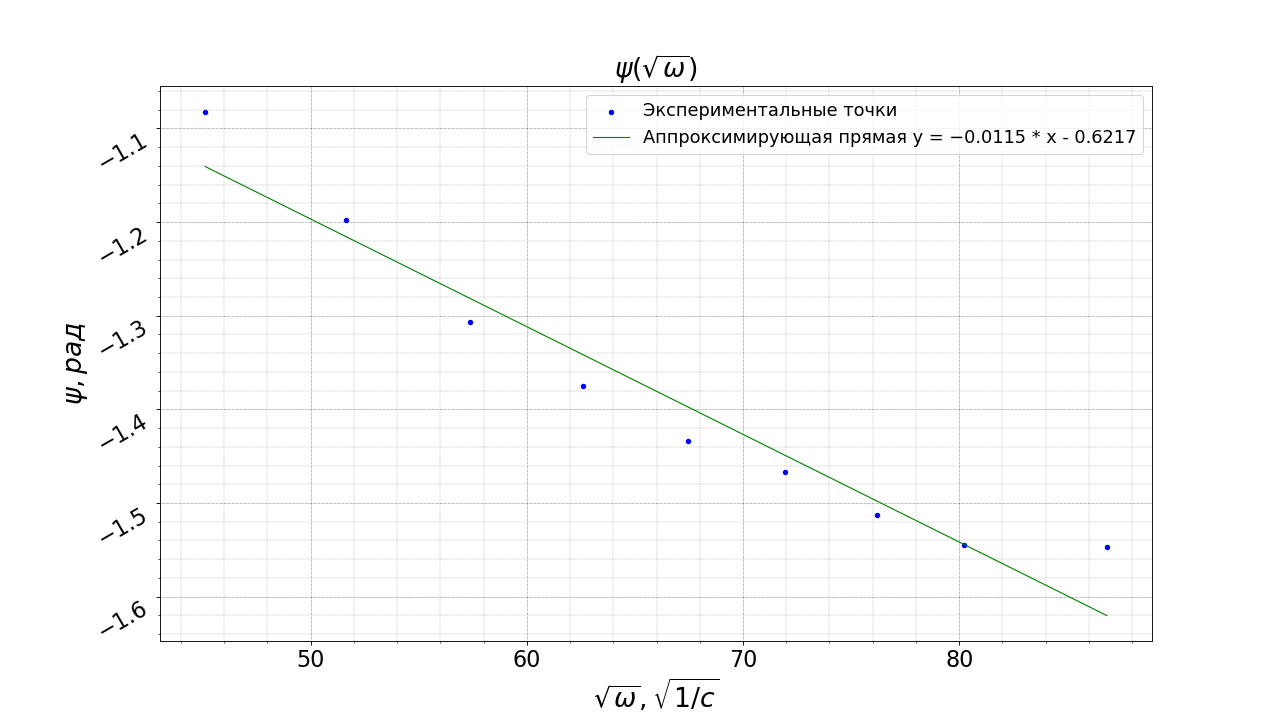
\includegraphics[width = 0.9\textwidth]{images/graph_2.png}
    \end{center}

    \noindent\hypertarget{graph_3}{\textbf{График 3.}}
    \begin{center}
        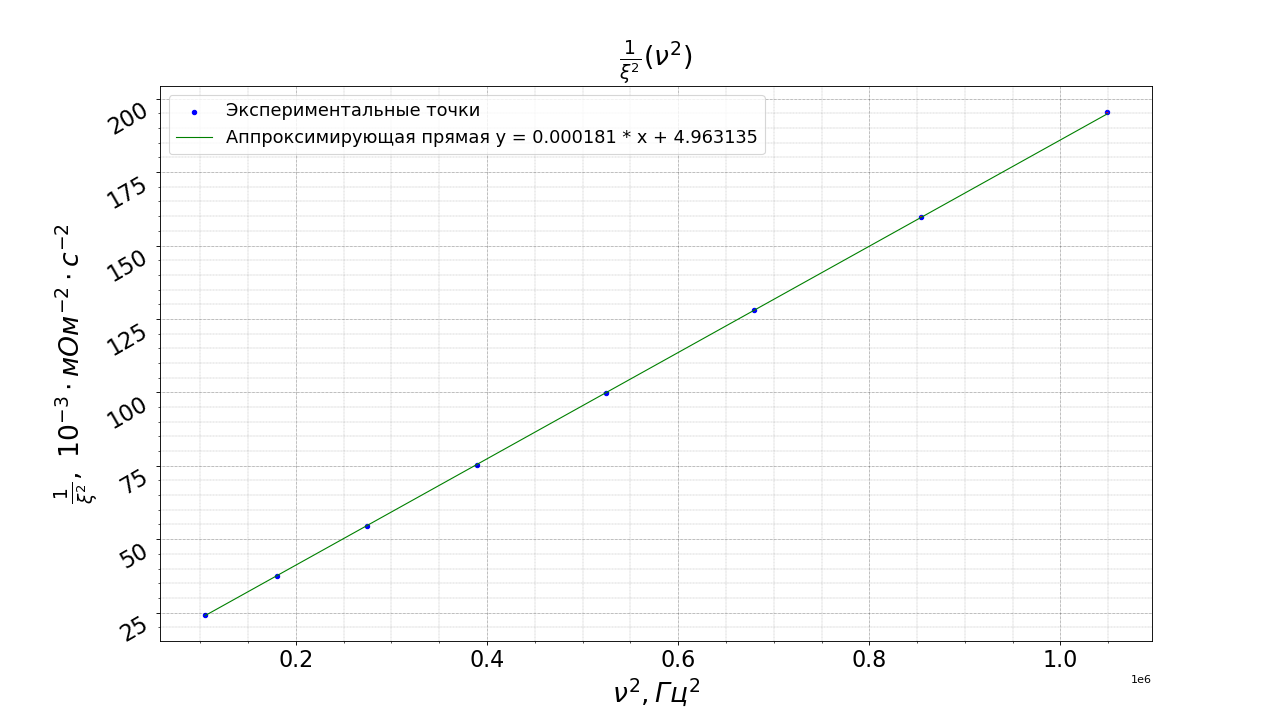
\includegraphics[width = 0.9\textwidth]{images/graph_3.png}
    \end{center}

    \noindent\hypertarget{graph_4}{\textbf{График 4.}}
    \begin{center}
        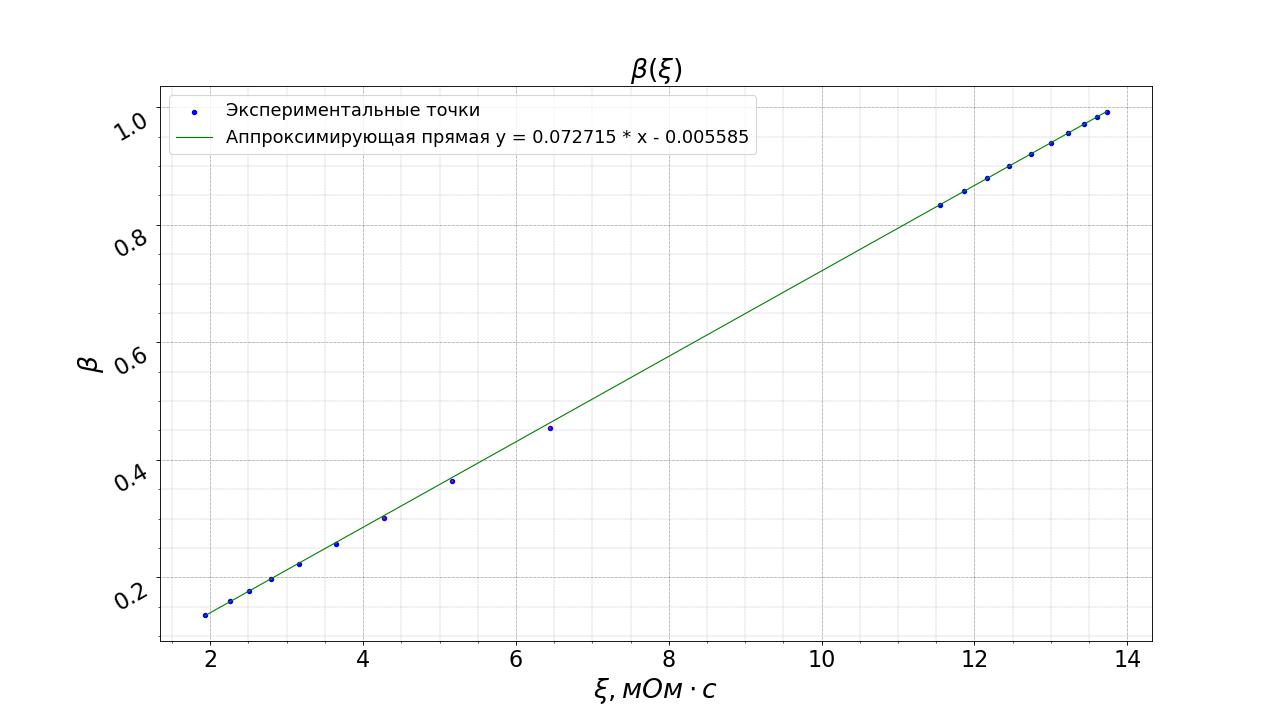
\includegraphics[width = 0.9\textwidth]{images/graph_4.png}
    \end{center}

\end{document}
